\documentclass[10pt, conference]{IEEEtran}
\IEEEoverridecommandlockouts

\usepackage{kotex}
\usepackage{cite}
\usepackage{amsmath,amssymb,amsfonts}
\usepackage{graphicx}
\usepackage{textcomp}
\usepackage{xcolor}
\usepackage{url}
\usepackage{booktabs}

% tighten float (figure/table) spacing to fit 2 pages
\setlength{\textfloatsep}{4pt plus 1pt minus 1pt}
\setlength{\floatsep}{4pt plus 1pt minus 1pt}
\setlength{\intextsep}{4pt plus 1pt minus 1pt}
\setlength{\dbltextfloatsep}{4pt plus 1pt minus 1pt}
\setlength{\abovecaptionskip}{2pt}
\setlength{\belowcaptionskip}{0pt}

\def\BibTeX{{\rm B\kern-.05em{\sc i\kern-.025em b}\kern-.08em
    T\kern-.1667em\lower.7ex\hbox{E}\kern-.125emX}}

\begin{document}

\title{에너지·해밍 지표를 통한\\
Posiform-Planted QUBO 벤치마크 난이도 분석}

\author{
\IEEEauthorblockN{김이든}
\IEEEauthorblockA{
컴퓨터공학과\\
강원대학교\\
춘천, 대한민국\\
이메일: rladlems1031@kangwon.ac.kr}
\and
\IEEEauthorblockN{이동재}
\IEEEauthorblockA{
융합보안학과\\
강원대학교\\
춘천, 대한민국\\
이메일: dongjae.lee@kangwon.ac.kr}
}

\maketitle

\begin{abstract}
QUBO 솔버(양자 어닐러와 고전 휴리스틱)를 평가하려면 정답을 미리 알면서도
풀기 어려운 인스턴스가 필요하다. Posiform 심기는 그런 인스턴스를 정답 하나를
심어 만든다. 최근 변형은 여기에 무작위 스핀글래스 항을 더하고, 심은 항을 계수
$\alpha$로 스케일해 난이도를 조절한다. 난이도는 보통 성공률로 매긴다. 즉 정확한
정답을 찾았는지를 본다. 그런데 어려운 영역 전체에서 이 값이 $0\%$다. 그래서
인스턴스·솔버·$\alpha$를 서로 가릴 수 없다. 우리는 대신 실패한 시도가 정답에
얼마나 가까운지를 잰다. 실패한 경우만, 가장 어려운 인스턴스를 고정한 집단에서,
두 가지 양을 기록한다. 하나는 정답까지의 에너지 차다. 다른 하나는 심은
정답으로부터의 해밍 거리(HD)다. 둘을 합치면 평평하던 $0\%$가 연속적인 난이도
곡선이 된다. D-Wave Pegasus 그래프($n{=}5612$)에서 시뮬레이티드 어닐링을 돌리면
곡선은 $\alpha$에 대해 비단조다. 정점까지 올랐다가 다시 내려간다. $\alpha$가
커질수록 실패 표본은 HD로는 가까워지지만 에너지로는 더 깊어진다. D-Wave
Advantage 어닐러에서의 한 번의 보조 실행도 같은 형태를 더 약하게 재현한다. 이는
그 구조가 SA만의 산물이 아님과 부합한다. 두 실패-조건부 지표를 함께 보고하면
성공률이 $0$인 영역에서도 posiform-planted QUBO 벤치마크를 더 세밀하게 평가할 수
있다.
\end{abstract}

\begin{IEEEkeywords}
QUBO 벤치마킹, posiform 심기, 양자 어닐링, 시뮬레이티드 어닐링,
해밍 거리, 에너지 차이, $\alpha$-난이도.
\end{IEEEkeywords}

\section{서론}
양자 어닐러와 고전 휴리스틱을 QUBO 문제로 평가하려면 최적해를 알면서도 찾기
어려운 인스턴스가 필요하다. Posiform 심기~\cite{hahn2023posiform}는 유일한 기저
상태를 갖는 QUBO를 만든다. 하지만 SA~\cite{kirkpatrick1983}로는 쉽게 풀린다.
Pelofske 등~\cite{pelofske2024hardened}은 이를 더 어렵게 만들었다. 무작위 이산계수
스핀글래스 QUBO $R_i$ 여러 개를 유일 최소해 $x^\star$인 posiform-planted QUBO
$P$에 계수 $\alpha$로 결합한다:
\begin{equation}
  Q_{\alpha}(x) \;=\; \sum_{i} R_{i}(x) \;+\; \alpha\,P(x).
  \label{eq:qalpha}
\end{equation}
그 연구는 난이도를 주로 무작위 QUBO 크기와 어닐링 시간으로 조절했다. $\alpha$는
$\{0.01,0.1\}$로 고정하고 기저상태 성공률을 보고했다. 그러나 성공률은 작은
$\alpha$ 영역 전체에서 $0\%$다. 그래서 그 영역 안의 인스턴스·솔버·$\alpha$ 값을
비교해 순위를 매길 수 없다. Pelofske 등도 성공률이 일률적으로 $0$인 구성에서는
에너지 차를 그림 하나로만 보고한다(그들의 Fig.~6, $\alpha{=}0.01$ 고정, 무작위
QUBO 크기에 대한 것). 그리고 난이도가 기저상태에 에너지가 매우 가까운 다수의 지역
최소에서 온다고 추정한다.

본 연구는 그 추정을 정량화한다. 에너지 차 $\Delta E = E - E_\text{target}$는
국소최소의 깊이를 나타낸다. 하지만 전체 표본에서 재면 깊이와 성공률이 뒤섞인다.
그래서 우리는 실패한 경우만 측정한다. 또 $\alpha$가 커지며 실패 집단이 바뀌는
것을 막으려고 가장 어려운 $100$개 인스턴스를 $\alpha$ 전역에서 고정한다. 이렇게
재면 오답만의 $\Delta E$와 해밍 거리(HD)가 $\Delta R{+}\alpha\,\Delta P$ 구조와
비단조 정점을 드러낸다. 두 지표 자체는 새롭지 않다. 우리의 기여는 측정
프로토콜이다. 고정한 최난해 집단에서 실패-조건부로 재면 무의미하던 $0\%$ 성공률이
순위를 매길 수 있는 곡선이 된다. 그리고 그 구조는 양자 어닐러에서의 한 번의 보조
실행으로도 재현되어, SA 구현만이 아니라 인스턴스를 반영함과 부합한다.

\section{방법론}
\textbf{인스턴스.} D-Wave Pegasus P16 그래프~\cite{boothby2020}($n{=}5612$ 큐비트)
위에 posiform-planted 인스턴스 $500$개를 생성한다. 각 계수 $R_{ij}$는 $-1$ 또는
$+1$이다. 그래프를 크기 $\leq 16$인 블록으로 재귀 이분할하고, 각 블록 $R_i$는
전수 탐색으로 푼다. 심은 정답 $x^\star$은 블록별 기저상태를 이어 붙인 것이다.
따라서 $\sum_i R_i$의 전역 최소해이기도 하다. $P$는 유일한 해가 $x^\star$인
2-SAT를 posiform으로 인코딩한 것이다. 난이도 분석에서는 $500$개 인스턴스를
$\alpha$ 전역의 SA 실패-읽기 총횟수로 순위 매긴다. 그중 가장 어려운 $100$개를
고정 집단으로 삼는다. 이 선정은 QPU 실행 전에 SA 결과만으로 한다. 그래서 아래의
솔버 간 일치는 순환논증이 아니다. 그런 다음 SA와 QPU를 모두 이 집단에 돌린다.

\textbf{지표.} 표본 $x$마다 HD$(x,x^\star)$~\cite{hamming1950}와 에너지 차
$\Delta E = E(x)-E(x^\star)\geq 0$를 같은 $Q_\alpha$ 기준으로 기록한다. 각
$R_{ij}$가 $\pm1$이라 모든 $R$ 에너지는 정수다. 그래서 $\Delta E$를 최소 비축퇴
$R$ 간격($\Delta_R{=}1$) 단위로 보고한다. 이 단위는 인스턴스마다 같고, HD$/n$도
그렇다. $\alpha{=}0$에서 $x^\star$은 $R$의 여러 기저상태 중 하나다. 그래서 에너지
일치($|\Delta E|<10^{-7}$)가 비트 일치는 아닐 수 있다. $\alpha{>}0$에선 기저상태가
유일하다. 우리는 성공을 비트 일치($x{=}x^\star$)로만 센다. $0\%$ 성공률과
per-read 실패율은 모두 $x^\star$의 정확 복원을 기준으로 하며, $\alpha{=}0$에서
축퇴인 에너지 기준이 아니다. 큰 $\alpha$에서 정답 표본($\Delta E{\approx}0$,
HD${=}0$)이 두 지표를 $0$으로 끌어내린다. 그래서 이하 통계는 모두 실패
조건부($x{\neq}x^\star$)로 낸다. 평균은 실패한 읽기에 대한 것이다. 인스턴스
$100$개 사이 표준오차는 SA에서 $0.06\,\Delta_R$ 미만이고, QPU에서도 정점
상승폭보다 훨씬 작아 오차 막대를 생략한다.

\textbf{프로토콜.} $\alpha$를 $0$, $10^{-9}$, $10^{-5}$, $10^{-4}$, $10^{-3}$,
$3{\times}10^{-3}$, $5{\times}10^{-3}$, $10^{-2}$, $1.5{\times}10^{-2}$,
$2{\times}10^{-2}$로 훑고, 정점 부근을 촘촘히 둔다. $2{\times}10^{-2}$보다 크면
어려운 집단마저 풀린다($\alpha{=}0.04$에서 읽기의 $19\%$만 실패). 그래서 고정된
실패 집단이 더는 없어 거기서 멈춘다(\S\ref{sec:vpc}). 주 실험은
\texttt{neal}~\cite{neal} SA 패키지를 (인스턴스,\,$\alpha$)당 $1000$ 스윕·$100$ 회
읽기로 돌린다. 또 $150$개 부분집합에서 $5000$ 스윕으로 $\Delta E$를 이진 성공률과
비교한다. 교차 확인을 위해 같은 $100$개를 D-Wave Advantage 어닐러에서 재실행한다.
minor-embedding 없이 하드웨어 네이티브로, 자동 스케일링·2-게이지 평균·$100$ 회
읽기·$20\,\mu$s 조건이다. $\Delta E$는 반환된 비트열에 원래 $Q_\alpha$를 적용해
다시 계산한다.

\section{결과}

\begin{figure}[!t]
\centering
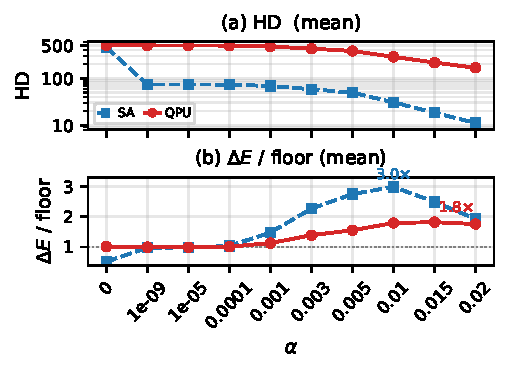
\includegraphics[width=\columnwidth]{figures/fig_sa_vs_qpu.pdf}
\caption{동일한 $100$개 최난해 인스턴스의 실패-조건부 난이도. 표시된 모든
$\alpha$에서 집단이 합산 읽기의 $\geq91\%$를 실패한다. 파랑: SA. 빨강: D-Wave
Advantage 어닐러. (a)~HD는 로그축이며 둘 다 단조 감소하나 $0$에 닿지 않는다.
(b)~$\Delta E$를 각 솔버의 작은 $\alpha$ floor(SA $\approx1.1\,\Delta_R$, QPU
$\approx24$)로 정규화해 한 축에 둔다. 둘 다 $1$에서 출발한다. SA는
$\alpha{=}10^{-2}$ 부근에서 정점 $3.0\times$까지 올랐다 내려간다. QPU는 같은
형태를 더 약하게($1.8\times$) 재현한다.}
\label{fig:traj}
\end{figure}

\begin{table}[!t]
\centering
\caption{동일한 $100$개 최난해 인스턴스의 오답만 평균 지표($\Delta E$는
$\Delta_R$ 단위). 표시된 모든 $\alpha$에서 SA는 집단 합산 실패율 $\geq91\%$,
QPU(D-Wave Advantage 어닐러)는 $0\%$ 성공. 정점 $\Delta E$ 굵게.}
\label{tab:metrics}
\footnotesize
\setlength{\tabcolsep}{5pt}
\renewcommand{\arraystretch}{1.0}
\begin{tabular}{lrrrr}
\toprule
 & \multicolumn{2}{c}{HD} & \multicolumn{2}{c}{$\Delta E$} \\
\cmidrule(lr){2-3}\cmidrule(lr){4-5}
$\alpha$ & SA & QPU & SA & QPU \\
\midrule
$0$               & 458.8 & 501.0 & 0.58 & 24.3 \\
$10^{-9}$         &  73.5 & 499.8 & 1.10 & 23.9 \\
$10^{-5}$         &  73.8 & 498.8 & 1.10 & 23.7 \\
$10^{-4}$         &  73.2 & 497.0 & 1.16 & 24.2 \\
$10^{-3}$         &  68.3 & 474.5 & 1.66 & 27.0 \\
$3\times10^{-3}$  &  58.4 & 427.2 & 2.54 & 33.3 \\
$5\times10^{-3}$  &  49.2 & 380.9 & 3.08 & 37.2 \\
$10^{-2}$         &  30.7 & 285.9 & \textbf{3.35} & 42.9 \\
$1.5\times10^{-2}$ & 18.4 & 216.1 & 2.79 & \textbf{43.5} \\
$2\times10^{-2}$  &  11.2 & 167.1 & 2.16 & 42.1 \\
\bottomrule
\end{tabular}
\end{table}

\subsection{$\alpha{=}0$의 축퇴와 HD}
순수 $R$에서는 표본의 $56.1\%$가 $R$의 기저상태에 정확히 도달한다(에너지 일치,
$\Delta E{=}0$). 하지만 $0\%$만 $x^\star$과 비트까지 일치하고, HD는 전역
최댓값($459$, $n$의 $8.2\%$)이다. 그래서 $\Delta E$는 두 갈래로 나뉜다. 중앙값은
$0$이지만 평균은 $0.58$이다. 들뜬 꼬리가 평균을 끌어올린다. $R$의 여러 기저상태가
정답과 에너지는 같으면서 비트로는 멀기 때문이다. 여기서 $E(x^\star)$은 이 축퇴
집합의 한 원소다. 그래서 $\Delta E$는 유일한 최적해가 아니라 그 기준까지의
거리이며, $\alpha{>}0$일 때와 의미가 다르다. $\Delta E$만 보면 $\alpha{=}0$을
풀린 것으로 판단할 수 있다. 그러나 어떤 표본도 정답 근처에 없음을 드러내는 것은
HD뿐이다. 두 지표가 모두 필요한 첫 번째 이유다.

\subsection{$\Delta E$의 바닥·정점·하강}
\label{sec:vpc}
고정 집단에서 오답만의 $\Delta E$는 $\Delta E = \Delta R + \alpha\,\Delta P$를
그대로 보여준다(표~\ref{tab:metrics}). 작은 $\alpha$ 구간($\alpha\in[10^{-9},10^{-4}]$)
에선 $\alpha\Delta P$가 무시할 만하다. 그래서 $\Delta E$가 순수 $R$의 국소최소
깊이에 평탄하게 머문다. 이 바닥값은 평균 $1.10$, 중앙값은 정확히 $1$(최소 $R$
간격 한 칸)이다. HD도 평탄하다($\approx73$). $\alpha$가 $10^{-3}$을 넘으면 심은
항이 두드러진다. $\Delta E$는 $1.66$($10^{-3}$)에서 $2.54$, $3.08$을 거쳐 올라
$\alpha{=}10^{-2}$에서 정점 $3.35$에 이른다. 이는 바닥의 $3.0$배다. 이후 다시
내려간다($2.79\to2.16$). 한편 HD는 전 구간에서 단조 감소한다($73\to11$). 즉 실패
표본은 $x^\star$에 비트로는 가까워지면서 에너지로는 더 깊어진다. 같은 표본을 두고
HD와 $\Delta E$가 반대 방향을 가리킨다(그림~\ref{fig:traj}). 정점은
$\Delta E = \Delta R + \alpha\Delta P$에서 비롯된다. $\Delta R$과 $\Delta P$는
비트열마다 고정된 값이다. 실패 집단이 $x^\star$ 쪽으로 이동할수록 그 $\Delta P$가
줄어든다. 그래서 커지는 $\alpha$가 이 감소를 더는 앞지르지 못하는 지점에서
$\Delta E$가 정점을 이룬다. 이 정점은 생존편향이나 선정편향의 산물이 아니다.
집단은 모든 $\alpha$에서 계속 실패한다(합산 읽기의 $\geq91\%$). 같은 비단조 형태가
인스턴스 $500$개 전체에서도 나타난다(바닥 $\approx1.1$, 정점 $\approx3.0$). 최난해
집단 선정은 이를 더 뚜렷하게 만들 뿐이다.

\subsection{양자 어닐러 일치성 점검}
\label{sec:qpu}
보조 증거로서, 같은 고정 집단의 인스턴스
$100$개를 D-Wave Advantage 어닐러(\texttt{Advantage\_system6.4})에서 한 번
실행했다(그림~\ref{fig:traj}, 빨강).
어닐러도 모든 $\alpha$·모든 인스턴스에서 실패한다($0\%$ 성공). 그래도 실패-조건부
지표는 같은 형태다. $\Delta E$는 평탄한 바닥에서 $\alpha{=}10^{-2}$ 부근의 정점까지
올랐다 내려간다. HD는 단조 감소한다($501\to167$). 바닥값은 SA보다 한 자릿수
크다($\Delta E\approx24$ 대 $1$, HD$\approx500$ 대 $73$). 즉 어닐러는 $x^\star$에서
훨씬 멀리 멈춘다. 정점도 상대적으로 더 약하다. floor의 $1.8\times$로, SA의
$3.0\times$에 못 미친다. 한 번의 실행으로 일반성을 확립할 수는 없다. 그래도 이는
그 구조가 SA 고유의 것이 아니라 인스턴스의 성질임과 부합한다. 정점에서 심은
커플러는 Ising 결합 $J\approx0.03$에 해당한다. 이는 소자의 통합 제어 오차(ICE)에
가깝다. 우리는 문제 스케일을 줄이면 이들이 ICE 아래로 내려가 정점이 평탄해지리라
본다. 이는 향후 과제로 남긴다.

\section{논의 및 결론}
갇힌 영역 전반에서 난이도를 진단하는 것은 오답만의 $\Delta E$이고, HD가 이를
보완한다. 둘은 서로가 놓치는 것을 잡아낸다. $\alpha{=}0$에서는 $\Delta E$의 중앙값
$0$이 풀린 것으로 오판하게 하는데, $R$의 축퇴를 HD의 최댓값이 드러낸다. 큰
$\alpha$에서는 HD의 감소가 진행을 보여준다. 전체 표본 평균, 즉 성공률은 이 정점을
가린다. 큰 $\alpha$에서 평균이 $\approx0$으로 떨어지는 것은 단지 더 많은 읽기가
성공해서다. 남은 실패는 여전히 깊다. $\Delta E$는 성공률로는 못 가르는 솔버도
구별한다. 앞의 최난해 $100$개와 다른 별도 $150$개 부분집합에서, $\alpha{=}10^{-3}$일
때 $1000$ 스윕과 $5000$ 스윕은 둘 다 성공률 $0\%$다. 그러나 평균 $\Delta E$는
$1.68$ 대 $1.00$으로 갈린다. 이 곡선은 SA 예산 전반에서 지속되고 보조 QPU
실행에서도 되풀이된다. 그래서 $\alpha$ 같은 난이도 매개변수를 훑을 때에는 고정한
최난해 집단에서 실패-조건부 $\Delta E$(바닥과 정점)를 HD와 함께 보고할 것을
권한다. 이렇게 하면 단일 난이도 점수가 아니라 벤치마크 인스턴스에 대한 실패-조건부
진단이 된다. 절대값은 솔버와 스케줄에 의존한다.

\textbf{한계.} QPU 증거는 단일 실행이다(2-게이지, 단일 $20\,\mu$s 어닐). 고전
쪽은 단일 SA 계열이다. 인스턴스는 단일 계수 타입($\pm1$)과 단일
토폴로지(Pegasus)를 쓴다.

\textbf{향후 과제.} 더 넓은 고전 솔버, 더 많은 어닐러 게이지와 다양한 어닐링
시간, 다른 계수 타입과 토폴로지, 그리고 HD와 $\Delta E$의 결합 분포 분석이다.
코드와 인스턴스는 \url{https://github.com/YIDEUNKIM/qubo_dataset}에서
공개한다.

\bibliographystyle{IEEEtran}
\begin{thebibliography}{99}

\bibitem{hahn2023posiform}
G.~Hahn, E.~Pelofske, and H.~N.~Djidjev,
``Posiform planting: generating QUBO instances with planted solutions for benchmarking,''
arXiv:2308.05859, 2023.

\bibitem{kirkpatrick1983}
S.~Kirkpatrick, C.~D.~Gelatt, and M.~P.~Vecchi,
``Optimization by simulated annealing,''
\emph{Science}, vol.~220, no.~4598, pp.~671--680, 1983.

\bibitem{pelofske2024hardened}
E.~Pelofske, G.~Hahn, and H.~N.~Djidjev,
``Increasing the hardness of posiform planting using random QUBOs for programmable quantum annealer benchmarking,''
\emph{npj Unconventional Computing}, vol.~2, art.~17, 2025
(arXiv:2411.03626).

\bibitem{boothby2020}
K.~Boothby, P.~Bunyk, J.~Raymond, and A.~Roy,
``Next-generation topology of D-Wave quantum processors,''
arXiv:2003.00133, 2020.

\bibitem{hamming1950}
R.~W.~Hamming, ``Error detecting and error correcting codes,''
\emph{Bell Syst.\ Tech.\ J.}, vol.~29, no.~2, pp.~147--160, 1950.

\bibitem{neal}
D-Wave Systems, ``\texttt{neal}: simulated annealing sampler,'' 2023.
\url{https://github.com/dwavesystems/dwave-neal}

\end{thebibliography}

\end{document}
